\section{Eigenvalues and Singular Values}
\subsection{}
\begin{definition}
  Let $A$ be an $nxn$ matrix. A scalar $\lambda$ is an eigenvalue of $A$ if 
  \[
  A\vec{v}=\lambda\vec{v}
  .\] 
  For some nonzero vector $\vec{v}\cdot\vec{v}$ is called the eigen vector corresponding to lambda.
\end{definition}
\begin{eg}
  Consider $A=\SmallMatrix{2&1\\1&2}$. Let's find the eigenvalues of this matrix.
    \begin{align*}
    0 &= det\left( \begin{pmatrix}2&1\\1&2\end{pmatrix}-\begin{pmatrix}\lambda&0\\0&\lambda\end{pmatrix}\right) \\
      &=det\begin{pmatrix} 2-\lambda&1\\1&2-\lambda \end{pmatrix} \\
      &=(2-\lambda)^2-1\\
    0&=(3-\lambda)(1-\lambda).
    \end{align*}
  Our eigenvalues are 3 and 1. Remember that $(A-\lambda I)\vec{v}=\vec{0}$. Consider $\lambda = 3$
  \begin{align*}
    \begin{pmatrix} -1&1\\1&-1 \end{pmatrix} \begin{pmatrix} x\\y \end{pmatrix} =\begin{pmatrix} 0\\0 \end{pmatrix} \\
    -x+y=0\\
    x=y\\
    \begin{pmatrix} x\\x \end{pmatrix} =x\begin{pmatrix} 1\\1 \end{pmatrix} 
  .\end{align*}
  Now consider $\lambda = 1$.
  \begin{align*}
    A(\lambda I)\vec{v}=\vec{0}\\
    (A-\lambda I)\vec{v}\\
    \begin{pmatrix} 1&1\\1&1 \end{pmatrix} \begin{pmatrix} x\\y \end{pmatrix} =\begin{pmatrix} 0\\0 \end{pmatrix} \\
    x+y=0\\
    y=-x\\
    \begin{pmatrix} x\\-x \end{pmatrix} =x\begin{pmatrix} 1\\-1 \end{pmatrix} 
  .\end{align*}
\end{eg}

\begin{eg}
  Consider $A=\SmallMatrix{1&1&2\\0&1&2\\0&0&3}\begin{pmatrix}1&1&2\\0&1&2\\0&0&3\end{pmatrix}$. For eigenvalues, $0=det(A-\lambda I)$.
  \begin{align*}
    0 = det \begin{pmatrix} 1-\lambda&1&2\\0&1-\lambda&2\\0&0&3-\lambda \end{pmatrix} \\
    0=(1-\lambda)(1-\lambda)(3-\lambda)
  .\end{align*}
  This makes our eigenvalues 1 and 3. For $\lambda=3$,
  \begin{align*}
    \begin{pmatrix} -2&1&2\\0&-2&2\\0&0&0 \end{pmatrix} \begin{pmatrix} x\\y\\z \end{pmatrix} &=\begin{pmatrix} 0\\0\\0 \end{pmatrix} \\
    -2y+2z&=0\\
    y&=0\\
    -2x+z+2z&=0\\
    -2x+3z&=0\\
    3z&=2x\\
    y&=z=\frac{2}{3}
  .\end{align*}
  This would make our eigenvector 
  \[
  \begin{pmatrix} x\\\frac{2}{3}x\\\frac{2}{3}x \end{pmatrix} =x\begin{pmatrix} 1\\\frac{2}{3}\\\frac{2}{3} \end{pmatrix} 
  .\] 
\end{eg}
\begin{definition}
  Given an eigenvalue $\lambda$ of $A$, the corresponding eigenvectors form a subspace denoted $v_\lambda$. Note that $v_\lambda=ker(A-\lambda I)$
\end{definition}
\begin{note}
  $\lambda=0$ is an eigenvalue of $A$ if and only if the $ker(A-\lambda I)=ker(A)=v_0\neq \{0\}$. This is true if and only if $A$ is singular ($det(A)=0$).
\end{note}
\begin{eg}
  Consider $\begin{pmatrix} 1&1\\1&1 \end{pmatrix} $. The determinant of 
  \[
    \begin{pmatrix} 1-\lambda&1\\1&1-\lambda \end{pmatrix} 
  \] 
  is equal to zero. We can see that when $\lambda =0$, the determinant is zero.
\end{eg}
\begin{prop}
  If $A$ is a real matrix and $\lambda+i\mu$ is an eigenvalue of $A$ with eigenvector $\vec{v}=\vec{x}+i\vec{y}$, then $\lambda-i\mu$ is an eigenvalue of $A$ with eigenvector $\vec{x}-i\vec{y}$.
\end{prop}
\begin{eg}
  Consider the matrix $A=\begin{bmatrix} 0&-1\\1&0 \end{bmatrix} $.
  \begin{align*}
    | A-\lambda I| = 0\\
    \left| \begin{matrix} -\lambda&-1\\1&-\lambda \end{matrix} \right| =0\\
    \lambda^2+1=0\\
    \lambda^2 = -1\\
    \lambda = \pm i = 0\pm i\\
    (A-\lambda I) \vec{v} = 0\\
    \begin{pmatrix} -i&-1\\1&-i \end{pmatrix} \begin{pmatrix} x\\y \end{pmatrix} =\begin{pmatrix} 0\\0 \end{pmatrix} \\
    -ix-y=0\\
    -ix=y
  .\end{align*}
  We now know that if we let $x$ be anything, and $y=-ix$, then we have the eigenvector. We can rewrite it as 
  \begin{align*}
    \begin{pmatrix} x\\-ix \end{pmatrix} =\boxed{} + i\boxed{}\\
    =\begin{pmatrix} x\\0 \end{pmatrix}+\begin{pmatrix} 0\\-ix \end{pmatrix}\\
    =x\begin{pmatrix} 1\\0 \end{pmatrix}+x\begin{pmatrix} 0\\-i \end{pmatrix}  \\
    =x\begin{pmatrix} 1\\0 \end{pmatrix} + i\begin{pmatrix} 0\\-1 \end{pmatrix} 
  .\end{align*}
  Now we also know that if $\lambda  = -i$ then the eigenvector is 
  \[
  \begin{pmatrix} 1\\0 \end{pmatrix} -i\begin{pmatrix} 0\\1 \end{pmatrix} 
  .\] 
\end{eg}
\lecture{1}{Monday March 29, 2021}{8.2, 8.3}
If $A$ is an $n\times n$ matrix with real entries, then 
\[
  det(A-\lambda I) = p(\lambda)= \text{The characteristic polynomial}
.\] 
\begin{note}
  If $A$ is $2\times 2$, then $P_A(\lambda)=\lambda^2-Tr(A)+det(A)$
\end{note}
Suppose that $A=\begin{bmatrix} a&b\\c&d \end{bmatrix}$. The trace ($Tr(A)$) is $=a+d$, and the determinant if $A$ is $ad-bc$, so 
\begin{align*}
  p_a(\lambda)=\left| \begin{matrix} a-\lambda&b\\c&d-\lambda \end{matrix} \right| 
  =(a-\lambda)(d-\lambda)-bc\\
  =ad-d\lambda-a\lambda+\lambda^2-bc\\
  =\lambda^2-(a+d)\lambda+(ad-bc)
.\end{align*}
Remember, the trace is $a+d$, and the determinant is $ad-bc$. Recall that $A$ is real, so $P_A(\lambda)$ is real. If we set $P_A(\lambda)=0$. By the fundamental theorem of algebra, $P_A(\lambda)$ factors into linear factors over $\C$. Consider the equation 
\[
x^{10}-7x^{9}+8x^2+\frac{1}{2}=0
.\] 
This factors into 10 different roots. So if $A$ is $n\times n$, $P_A(\lambda)$ has at most $n$ roots in $\C$
\begin{theorem}
  Let $A$ be $n\times n$ with real entries. Then $A$ has at most $n$ eigenvalues. If $a+bi$ is an eigenvalue, then so is $a-bi$
\end{theorem}
\begin{eg}
  The Jordan Block Matrix. Let's look at $J_{2,3}=\begin{bmatrix} 2&1&0\\0&2&1\\0&0&2 \end{bmatrix} $. Let's find the eigenvalues:
  \begin{align*}
    | J_{2,3}-\lambda I| = 0\\
    \left| \begin{matrix} 2-\lambda&1&0\\0&2-\lambda&1\\0&0&2-\lambda \end{matrix} \right| =0\\
    (2-\lambda)(2-\lambda)(1-\lambda)=0\\
    \lambda=2
  .\end{align*}
  Now let's find the eigenvector(s):
  \begin{align*}
    (a-lambda I)\vec{v}=\vec{0}\\
    \begin{pmatrix} 0&1&0\\0&0&1\\0&0&0 \end{pmatrix} \begin{pmatrix} x\\y\\z \end{pmatrix} =\begin{pmatrix} 0\\0\\0 \end{pmatrix} \\
    y=0\\
    z=0\\
    \begin{pmatrix} x\\0\\0 \end{pmatrix} =x\begin{pmatrix} 1\\0\\0 \end{pmatrix} 
  .\end{align*}
\end{eg}
\begin{theorem}
  If $A$ is square, then $P_A(\lambda)=P_{A^{T}}(\lambda)$. So, $A$ and $A^{T}$ have the same eigenvalues. Probably not the same eigenvectors.
\end{theorem}
\begin{theorem}
  Let $A$ be $n\times n$. The sum of the eigenvalues of $A$ is equal to the $Tr(A)$, and the product of the eigenvalues of $A$ is equal to $det(A)$.
\end{theorem}
\begin{eg}
  $J_{2,3}=\begin{pmatrix} 2&1&0\\0&2&1\\0&0&2 \end{pmatrix} $. The Trace of $J_{2,3}=2+2+2$ (adding the diagonals). The determinant of $J_{2,3}=2*2*2$ (multiplication of the diagonals).
  \[
    P_{J_{2,3}}(\lambda)=(2-\lambda)(2-\lambda)(2-\lambda)
  .\] 
\end{eg}
\subsection{}
\begin{prop}
  If $\lambda_1,\ldots,\lambda_k$ are distinct eigenvalues of $A,$ then the corresponding eigenvectors are linearly independent.
\end{prop}
\begin{eg}
  Let's let $A=\begin{bmatrix} 1&1&0\\0&2&-1\\0&0&3 \end{bmatrix} $. Let's find the eigenvalues of $A$.
  \begin{align*}
    0=P_A(\lambda) &= \left| \begin{matrix} 1-\lambda&1&0\\0&2-\lambda&-1\\0&0&3-\lambda \end{matrix} \right| \\
    0&=(1-\lambda)(2-\lambda)(3-\lambda)\\
    \lambda&=1,2,3
  .\end{align*}
  For $\lambda=1$
  \begin{align*}
    (A-\lambda I)\vec{v}&=\vec{0}\\
    \begin{pmatrix} 0&1&0\\0&1&-1\\0&0&2 \end{pmatrix} \begin{pmatrix} x\\y\\z \end{pmatrix} &=\begin{pmatrix} 0\\0\\0 \end{pmatrix} \\
    y&=0\\
    y-z&=0\\
    z&=0\\
    \begin{pmatrix} x\\0\\0 \end{pmatrix} &=x\begin{pmatrix} 1\\0\\0 \end{pmatrix} 
  .\end{align*}
  Now for $\lambda=2$
  \begin{align*}
    \begin{pmatrix} -1&1&0\\0&0&-1\\0&0&1 \end{pmatrix} \begin{pmatrix} x\\y\\z \end{pmatrix} &=\begin{pmatrix} 0\\0\\0 \end{pmatrix} \\
    -x+y&=0\\
    x&=y
    -z&=0\\
    \begin{pmatrix} x\\x\\0 \end{pmatrix} &=x\begin{pmatrix} 1\\1\\0 \end{pmatrix} 
  .\end{align*}
  Now for $\lambda=3$
  \begin{align*}
    \begin{pmatrix} -2&1&0\\0&-1&-1\\0&0&0 \end{pmatrix} \begin{pmatrix} x\\y\\z \end{pmatrix} &=\begin{pmatrix} 0\\0\\0 \end{pmatrix} \\
    -2x+y&=0\to y=2x\\
    -y-z&=0\to z=-y\\
    z&=-2x\\
    \begin{pmatrix} x\\2x\\-2x \end{pmatrix} &=x\begin{pmatrix} 1\\2\\-2 \end{pmatrix} 
  .\end{align*}
  We now have the following eigenvectors 
  \[
  \begin{pmatrix} 1\\0\\0 \end{pmatrix} ,\begin{pmatrix} 1\\1\\0 \end{pmatrix} ,\begin{pmatrix} 1\\2\\-2 \end{pmatrix} 
  .\] 
  These are linearly independent so we have a basis for $\R^3$
\end{eg}
\begin{theorem}
  If $A$ is $n\times n$ and $a$ has $n$ distinct real (/complex) eigenvalues, then the corresponding eigenvectors form a basis for $\R^b(\C^n)$. 
\end{theorem}
Now\ldots vector spaces. Vectors have two main operations,
\begin{align*}
  \vec{v}+\vec{w}\\
  c\cdot v
.\end{align*}
Let $V, W$ be vector spaces over $\R$. We know that $\R^3\begin{pmatrix} a\\0\\0 \end{pmatrix}$. In reality, $V, W$ are the same, but we must show that they are the same. We would need a function that preserves the operations from $V$ to $W$. A map (function) $f$ from $V$ to $W$ should have the following
\begin{align*}
  f(\vec{v_1}+\vec{v_2})&=f(\vec{v_1})+f(\vec{v_2})\\
  f(r\cdot \vec{v})&=rf(\vec{v})
.\end{align*}
\lecture{2}{Wednesday, March 31st}{8.3}
Recall that $\lambda=0$ is an eigenvalue of $A$, if and only if
\[
  (A-0\cdot I)\vec{v}=\vec{0}
\] has a $\vec{v}\neq \vec{0}$ solution if and only if 
\[
  ker(A)\neq\{0\}
\] if and only if  $A^{-1}$ does not exist.
\begin{theorem}
  If $\lambda_1,\ldots,\lambda_k$ are distinct eigenvalues of $A$, then the corresponding eigenvectors are linearly independent.
\end{theorem}
\begin{eg}
  Consider $A=\begin{pmatrix} 2&1\\1&2 \end{pmatrix} $. The eigenvalues for this matrix are $\lambda=3,1$. The eigenvector for $\lambda=3$ is $\begin{pmatrix} 1\\1 \end{pmatrix} $, and the eigenvector for $\lambda=1$ is $\begin{pmatrix} -1\\1 \end{pmatrix} $.
\end{eg}
\begin{eg}
  Consider $A=\begin{pmatrix} 1&1&2\\0&1&2\\0&0&3 \end{pmatrix} $. The characteristic polynomial is $P(\lambda)=(1-\lambda)^2(3-\lambda)$. For $ \lambda = 1$, the eigenvector is $\begin{pmatrix} 1\\0\\0 \end{pmatrix} $, and for $\lambda = 3$, the eigenvector is $\begin{pmatrix} 3\\2\\2 \end{pmatrix} $ 
\end{eg}
\begin{theorem}
  If $A $ is $n\times n$ and $A$ has $n$ distinct real (or complex) eigenvalues, then the corresponding eigenvectors $\vec{v_1},\ldots,\vec{v_n}$ form a basis for $\R^{n}$.
\end{theorem}
  Consider $A=\begin{pmatrix} 1&-1\\2&4 \end{pmatrix} $. $A$ defines a map from $\R^{2}$ to $\R^2$. Our map is 
  \begin{align*}
    L: \begin{pmatrix} x\\y \end{pmatrix}\to A\begin{pmatrix} x\\y \end{pmatrix}\\
    L\left( r\vec{v} \right) =rL(\vec{v})
  .\end{align*}
  $L$ is a linear transformation.

\begin{eg}
  Consider $A=\begin{pmatrix} 1&-1\\2&4 \end{pmatrix} $. What happens if we multiply $A$ by $\begin{pmatrix} 2\\1 \end{pmatrix} $?
  \begin{align*}
    A\begin{pmatrix} 2\\1 \end{pmatrix} =\begin{pmatrix} 1&-1\\2&4 \end{pmatrix} \begin{pmatrix} 2\\1 \end{pmatrix} \\
    =\begin{pmatrix} 1\\8 \end{pmatrix} 
  .\end{align*}
  Let's think of $\begin{pmatrix} 2\\1 \end{pmatrix} $ as $2e_1+1e_2$. This would make our equation \[
  2\begin{pmatrix} 1\\0 \end{pmatrix} +\begin{pmatrix} 0\\1 \end{pmatrix} 
  .\] 
  Let's also think about $\begin{pmatrix} 1\\8 \end{pmatrix} $ as \[
  1\begin{pmatrix} 1\\0 \end{pmatrix} +8\begin{pmatrix} 0\\1 \end{pmatrix} 
  .\] 
  We can change the basis to 
  \begin{align*}
    v_1=\begin{pmatrix} 1\\-1 \end{pmatrix} && v_2=\begin{pmatrix} 1\\-2 \end{pmatrix} 
  .\end{align*}
\end{eg}
\lecture{3}{Monday March 29, 2021}{8.2, 8.3}

\begin{figure}[h]
  \centering
  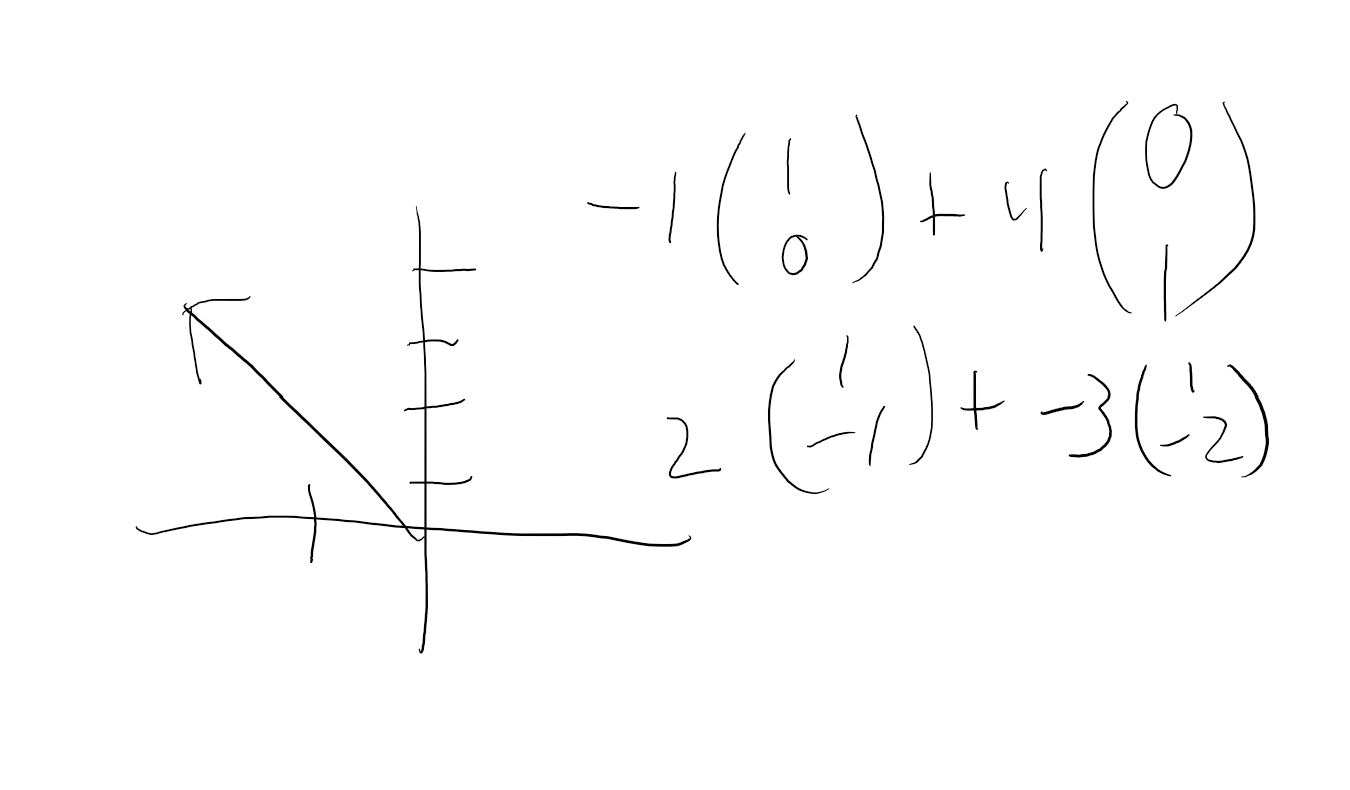
\includegraphics[width=0.8\textwidth]{resource/images/8-2Figure1.png}
  \caption{Example Line image}
  \label{fig:}
\end{figure}

A linear transformation consists of the following:
\begin{align*}
  L(v_1+v_2)&=L(v_1)+L(v_2)\\
  L(r\cdot v)&=rL(v)
.\end{align*}
  Consider $A = \begin{pmatrix} 1&-1\\2&4 \end{pmatrix} $. If everything is in the standard basis then 
  \begin{align*}
    \begin{pmatrix} 1&-1\\2&4 \end{pmatrix} \begin{pmatrix} -1\\4 \end{pmatrix} =\begin{pmatrix} -5\\14 \end{pmatrix} \\
    -1\begin{pmatrix} 1\\0 \end{pmatrix} + 4\begin{pmatrix} 0\\1 \end{pmatrix} \to -5\begin{pmatrix} 1\\0 \end{pmatrix} +14\begin{pmatrix} 0\\1 \end{pmatrix} 
  .\end{align*}
  It's harder to figure out what the vector is with the new basis from the picture, but the transformation has a nice description of \[
    B=\begin{pmatrix} 2&0\\0&3 \end{pmatrix} 
  .\] 
  If we take $B$ and hit it with the new coefficients:
  \begin{align*}
    \begin{pmatrix} 2&0\\0&3 \end{pmatrix} \begin{pmatrix} 2\\-3 \end{pmatrix} =\begin{pmatrix} 4\\-9 \end{pmatrix} \\
    2\begin{pmatrix} 1\\-1 \end{pmatrix} + -3\begin{pmatrix} 1\\-2 \end{pmatrix} \to 4\begin{pmatrix} 1\\-1 \end{pmatrix} +-9\begin{pmatrix} 1\\-2 \end{pmatrix} 
  .\end{align*}
    The left hand side is equal to $\begin{pmatrix} -1\\4 \end{pmatrix}$ and the right hand side is equal to $\begin{pmatrix} -5\\14 \end{pmatrix}$ If we take $\begin{pmatrix} 2&0\\0&3 \end{pmatrix} \begin{pmatrix} 1\\0 \end{pmatrix} =\begin{pmatrix} 2\\0 \end{pmatrix} $, which looks like an eigenvector. The first basis that we had was $\left\{\begin{pmatrix} 1\\0 \end{pmatrix}, \begin{pmatrix} 0\\1 \end{pmatrix}  \right\}$, and the second basis was $\left\{\begin{pmatrix} 1\\-1 \end{pmatrix}, \begin{pmatrix} 1\\-2 \end{pmatrix}  \right\}$. So we took basis 1 and did a linear transofrmation to get basis 2 like the following 
    \[
    \begin{pmatrix} 1&-1\\2&4 \end{pmatrix} \to \begin{pmatrix} 2&0\\0&3 \end{pmatrix} 
    .\] If $A$ is in the standard basis. Then $B=S^{-1}AS$, where $S=\begin{pmatrix} \vec{v_1},\vec{v_2},\ldots,\vec{v_{n}} \end{pmatrix} $, where $\{\vec{v_1},\ldots,\vec{v_n}\}$ is the new basis.
\begin{eg}
  Let $A=\begin{pmatrix} 1&-1\\2&4 \end{pmatrix} $.
  \begin{align*}
    S=\begin{pmatrix} 1&1\\-1&-2 \end{pmatrix} \\
    S^{-1}=\frac{1}{-2--1}\begin{pmatrix} -2&-1\\1&1 \end{pmatrix} \\
    =\begin{pmatrix} 2&1\\-1&-1 \end{pmatrix} \\
    B=S^{-1}AS=\begin{pmatrix} 2&1\\-1&-1 \end{pmatrix} \begin{pmatrix} 1&-1\\2&4 \end{pmatrix} \begin{pmatrix} 1&1\\-1&-2 \end{pmatrix} \\
    = \begin{pmatrix} 2&1\\-1&-1 \end{pmatrix} \begin{pmatrix} 2&3\\-2&-6 \end{pmatrix} \\
    =\begin{pmatrix} 2&0\\0&3 \end{pmatrix} 
  .\end{align*}
\end{eg}
\begin{definition}
  A square matrix $A$ is diagonalizable if there is a matrix $S$ and a diagonal matrix $\Lambda$ such that 
  \begin{equation*}
    \Lambda = S^{-1}AS
  \end{equation*}
\end{definition}
\begin{theorem}
  $A$ is diagonalizable if and only if $A$ has $n$ linearly independent eigenvectors $\vec{v_1},\ldots,\vec{v_n}$. In this case, \[
  \Lambda = S^{-1}AS
  .\] where $S=\begin{bmatrix} \vec{v_1},\ldots,\vec{v_n} \end{bmatrix} $, and $\Lambda=\begin{bmatrix} \lambda_1&0\\0&\lambda_n \end{bmatrix} $, where $\lambda_i$ is the eigenvalue for $\vec{v_i}$
\end{theorem}
If we are looking for the linearly independent solutions we need to do $A-\lambda I=0$. From here we would get lambda values and create eigenvectors using $A-\lambda I\vec{v}=0$
\begin{eg}
  Let $A=\begin{pmatrix} 0&-1&-1\\1&2&1\\1&1&2 \end{pmatrix} $, which is our standard matrix. Once we find our \[
  \Lambda = \begin{pmatrix} 1&0&0\\0&1&0\\0&0&2 \end{pmatrix} 
  .\] Our basis is \[
  \begin{pmatrix} -1\\1\\0 \end{pmatrix} \begin{pmatrix} -1\\0\\1 \end{pmatrix} \begin{pmatrix} -1\\1\\1 \end{pmatrix} 
  .\] Let's take $A$ and hit it with coefficients in the standard basis. Let's try \[
  A\cdot\begin{pmatrix} -3\\2\\2 \end{pmatrix} 
  .\] We need to think about the matrix on the right hand side as $-3\begin{pmatrix} 1\\0\\0 \end{pmatrix} +2\begin{pmatrix} 0\\1\\0 \end{pmatrix} +2\begin{pmatrix} 0\\0\\1 \end{pmatrix} $, so we can do the following:
  \begin{align*}
    \begin{pmatrix} 0&-1&-1\\1&2&1\\1&1&2 \end{pmatrix} \begin{pmatrix} -3\\2\\2 \end{pmatrix} =\begin{pmatrix} -4\\3\\3 \end{pmatrix} 
  .\end{align*}
  We know that our divided up equation from before (for the right matrix) is getting mapped to $4\begin{pmatrix} 1\\0\\0 \end{pmatrix} +3\begin{pmatrix} 0\\1\\0 \end{pmatrix} +3\begin{pmatrix} 0\\0\\1 \end{pmatrix} $. We know that our $\Lambda$ must take $\begin{pmatrix} -3\\2\\2 \end{pmatrix} $, but we need to rewrite it in our new basis.\[
  1\begin{pmatrix} -1\\1\\0 \end{pmatrix} +1\begin{pmatrix} -1\\0\\1 \end{pmatrix} +1\begin{pmatrix} -1\\1\\1 \end{pmatrix} 
  .\] 
  If we multiply this by our $\lambda$, we can figure out out map. \[
    \begin{pmatrix} 1&0&0\\0&1&0\\0&0&2 \end{pmatrix} \begin{pmatrix} 1\\1\\1 \end{pmatrix} =\begin{pmatrix} 1\\1\\2 \end{pmatrix} 
  .\] 
  Our equation gets mapped to \[
  1\begin{pmatrix} -1\\1\\0 \end{pmatrix} +1\begin{pmatrix} -1\\0\\1 \end{pmatrix} +2\begin{pmatrix} -1\\1\\1 \end{pmatrix} 
  .\] 
  This means that our vector is the same from before because we get $\begin{pmatrix} -4\\3\\3 \end{pmatrix} $.\newline
  $Av_1\to w_1$, while $\Lambda v_2\to w_2$.
\end{eg}

\lecture{4}{Monday April 12, 2021}{}

\lecture{5}{Wednesday April 14, 2021}{}

If we have an $n\times n$ matrix with $n$ distinct eigenvalues, we have $n$ linearly independent eigenvectors. \[
\Lambda=S^{-1}AS
.\] 
If the matrix is real symmetric, then we can get a real eigenvector basis so we can diagonalize like \[
S\Lambda S^{-1}=A
.\] 
If we do $A\cdot A$, then we get 
\begin{align*}
  S\Lambda S^{-1}S\Lambda S^{-1}\\
  =S \Lambda S^{-1}\\
  A^{k}=S \Lambda ^{k}S^{-1}
.\end{align*}
Let's look at an example where this is not going to work. 
\begin{eg}
  Let $M=\begin{bmatrix} 1&1&1\\0&1&0\\0&0&1 \end{bmatrix} $. This matrix only has one eigenvalue of $\lambda=1$. Let's find the eigenvectors.
  \begin{align*}
    \begin{bmatrix} 0&1&1\\0&0&0\\0&0&0 \end{bmatrix} \begin{bmatrix} x\\y\\z \end{bmatrix} =\begin{bmatrix} 0\\0\\0 \end{bmatrix} \\
    y+z=0\to z=-y\\
    \begin{bmatrix} x\\y\\-y \end{bmatrix} =x\begin{bmatrix} 1\\0\\0 \end{bmatrix} +y\begin{bmatrix} 0\\1\\-1 \end{bmatrix} 
  .\end{align*}
\end{eg}
Now supposed instead, if we let $M=\begin{bmatrix} 1&0&0\\0&1&0\\0&0&1 \end{bmatrix} $. This matrix must have 3 linearly independent eigenvectors.
\begin{align*}
  |M- \lambda I|=0\\
  \left| \begin{matrix} 1-\lambda &0&0\\0&1-\lambda&0\\0&0&1-\lambda \end{matrix} \right| =0\\
  (M-\lambda I)\vec{v} = 0\\
  \begin{bmatrix} 0&0&0\\0&0&0\\0&0&0 \end{bmatrix} \begin{bmatrix} x\\y\\z \end{bmatrix} =\begin{bmatrix} 0\\0\\0 \end{bmatrix} \\
  \begin{bmatrix} x\\y\\z \end{bmatrix} =x\begin{bmatrix} 1\\0\\0 \end{bmatrix} +y\begin{bmatrix} 0\\1\\0 \end{bmatrix} +z\begin{bmatrix} 0\\0\\1 \end{bmatrix} 
.\end{align*}

\begin{theorem}
  Let $A=A^{T}$ be an $n\times n$ real matrix. Let $\vec{v_1},\ldots,\vec{v_n}$ be an eigenvector basis such that $\vec{v_1},\ldots,\vec{v_r}$ correspond to nonzero eigenvalues and $\vec{v_{r+1}},\ldots,\vec{v_n}$ correspond to the zero eigenvalue. Then $r=rank(A)$, $\vec{v_1},\ldots,\vec{v_r}$ form an orthogonal basis for $IM(A)=coimg(A)$, and $\vec{v_{r+1}},\ldots,\vec{v_n}$ form an orthogonal basis for the $ker(A)=coker(A)$.
\end{theorem}
\begin{theorem}
  The spectral theorem. Let $A$ be a real symmetric matrix. Then there exists an orthogonal matrix $Q$ such that $A=Q\Lambda Q^{-1}=Q\Lambda Q^{T}$, where $\Lambda $ is a real diagonal matrix. The eigenvalues of $A$ appear on the diagonal of $\Lambda $, while the columns of $Q$ are orthonormal eigenvectors of $A$.
\end{theorem}
\begin{eg}
  Let $A=\begin{bmatrix} 1&-1&1\\-1&1&0\\1&01 \end{bmatrix} $. Our eigenvalues are $1+\sqrt{2},1,1-\sqrt{2}  $, which means our eigenvectors are \[
  \begin{bmatrix} \sqrt{2} \\-1\\1 \end{bmatrix} ,\begin{bmatrix} 0\\1\\1 \end{bmatrix} ,\begin{bmatrix} -\sqrt{2} \\-1\\1 \end{bmatrix} 
  .\] 
  The orthonormal basis of the eigenvectors is 
  \begin{align*}
    \sqrt{(\sqrt{2} )^2+(-1)^2+1^2}\\
    =\sqrt{6}\\
    \begin{bmatrix} \frac{\sqrt{2} }{2}\\-\frac{1}{2}\\\frac{1}{2} \end{bmatrix} ,\begin{bmatrix} 0\\\frac{1}{\sqrt{2} }\\\frac{1}{\sqrt{2} } \end{bmatrix} ,\begin{bmatrix} \frac{1}{2}\\\frac{1}{2}\\\frac{1}{2} \end{bmatrix} 
  .\end{align*}
  Now if we let $S=\begin{bmatrix} \sqrt{2} &0&-\sqrt{2}\\-1&1&-1\\1&1&1  \end{bmatrix} $ and we do \[
  S^{-1}AS= \Lambda=\begin{bmatrix} 1+\sqrt{2}&0&0\\0&1&0\\0&0&1-\sqrt{2}   \end{bmatrix} 
  .\] 
\end{eg}

\lecture{6}{Friday April 16}{8.6}
